% !TeX program = pdfLaTeX
% \documentclass[12pt]{article}
\documentclass[12pt, a4paper]{report} % fot TsukubaBP
\usepackage{amsmath}
\usepackage{graphicx,psfrag,epsf}
\usepackage{enumerate}
\usepackage{natbib}
\usepackage{textcomp}
\usepackage[hyphens]{url} % not crucial - just used below for the URL
\usepackage{hyperref}
\usepackage{longtable}
\providecommand{\tightlist}{%
  \setlength{\itemsep}{0pt}\setlength{\parskip}{0pt}}
\usepackage{setspace} % for TsukubaBP
\setstretch{1.6}      % for TsukubaBP
\usepackage{seqsplit} % for TsukubaBP

%\pdfminorversion=4

% DON'T change margins - should be 1 inch all around.
\addtolength{\oddsidemargin}{-.5in}%
\addtolength{\evensidemargin}{-.5in}%
\addtolength{\textwidth}{1in}%
\addtolength{\textheight}{1.3in}%
\addtolength{\topmargin}{-.8in}%
% \addtolength{\oddsidemargin}{0cm}   % for TsukubaBP
% \addtolength{\evensidemargin}{0cm}  % for TsukubaBP
% \addtolength{\textwidth}{16cm}      % for TsukubaBP
% \addtolength{\textheight}{23.7cm}   % for TsukubaBP
% \addtolength{\topmargin}{-45pt}     % for TsukubaBP


%% load any required packages here


\usepackage{color}
\usepackage{fancyvrb}
\newcommand{\VerbBar}{|}
\newcommand{\VERB}{\Verb[commandchars=\\\{\}]}
\DefineVerbatimEnvironment{Highlighting}{Verbatim}{commandchars=\\\{\}}
% Add ',fontsize=\small' for more characters per line
\usepackage{framed}
\definecolor{shadecolor}{RGB}{248,248,248}
\newenvironment{Shaded}{\begin{snugshade}}{\end{snugshade}}
\newcommand{\AlertTok}[1]{\textcolor[rgb]{0.94,0.16,0.16}{#1}}
\newcommand{\AnnotationTok}[1]{\textcolor[rgb]{0.56,0.35,0.01}{\textbf{\textit{#1}}}}
\newcommand{\AttributeTok}[1]{\textcolor[rgb]{0.77,0.63,0.00}{#1}}
\newcommand{\BaseNTok}[1]{\textcolor[rgb]{0.00,0.00,0.81}{#1}}
\newcommand{\BuiltInTok}[1]{#1}
\newcommand{\CharTok}[1]{\textcolor[rgb]{0.31,0.60,0.02}{#1}}
\newcommand{\CommentTok}[1]{\textcolor[rgb]{0.56,0.35,0.01}{\textit{#1}}}
\newcommand{\CommentVarTok}[1]{\textcolor[rgb]{0.56,0.35,0.01}{\textbf{\textit{#1}}}}
\newcommand{\ConstantTok}[1]{\textcolor[rgb]{0.00,0.00,0.00}{#1}}
\newcommand{\ControlFlowTok}[1]{\textcolor[rgb]{0.13,0.29,0.53}{\textbf{#1}}}
\newcommand{\DataTypeTok}[1]{\textcolor[rgb]{0.13,0.29,0.53}{#1}}
\newcommand{\DecValTok}[1]{\textcolor[rgb]{0.00,0.00,0.81}{#1}}
\newcommand{\DocumentationTok}[1]{\textcolor[rgb]{0.56,0.35,0.01}{\textbf{\textit{#1}}}}
\newcommand{\ErrorTok}[1]{\textcolor[rgb]{0.64,0.00,0.00}{\textbf{#1}}}
\newcommand{\ExtensionTok}[1]{#1}
\newcommand{\FloatTok}[1]{\textcolor[rgb]{0.00,0.00,0.81}{#1}}
\newcommand{\FunctionTok}[1]{\textcolor[rgb]{0.00,0.00,0.00}{#1}}
\newcommand{\ImportTok}[1]{#1}
\newcommand{\InformationTok}[1]{\textcolor[rgb]{0.56,0.35,0.01}{\textbf{\textit{#1}}}}
\newcommand{\KeywordTok}[1]{\textcolor[rgb]{0.13,0.29,0.53}{\textbf{#1}}}
\newcommand{\NormalTok}[1]{#1}
\newcommand{\OperatorTok}[1]{\textcolor[rgb]{0.81,0.36,0.00}{\textbf{#1}}}
\newcommand{\OtherTok}[1]{\textcolor[rgb]{0.56,0.35,0.01}{#1}}
\newcommand{\PreprocessorTok}[1]{\textcolor[rgb]{0.56,0.35,0.01}{\textit{#1}}}
\newcommand{\RegionMarkerTok}[1]{#1}
\newcommand{\SpecialCharTok}[1]{\textcolor[rgb]{0.00,0.00,0.00}{#1}}
\newcommand{\SpecialStringTok}[1]{\textcolor[rgb]{0.31,0.60,0.02}{#1}}
\newcommand{\StringTok}[1]{\textcolor[rgb]{0.31,0.60,0.02}{#1}}
\newcommand{\VariableTok}[1]{\textcolor[rgb]{0.00,0.00,0.00}{#1}}
\newcommand{\VerbatimStringTok}[1]{\textcolor[rgb]{0.31,0.60,0.02}{#1}}
\newcommand{\WarningTok}[1]{\textcolor[rgb]{0.56,0.35,0.01}{\textbf{\textit{#1}}}}

% Pandoc citation processing
\newlength{\csllabelwidth}
\setlength{\csllabelwidth}{3em}
\newlength{\cslhangindent}
\setlength{\cslhangindent}{1.5em}
% for Pandoc 2.8 to 2.10.1
\newenvironment{cslreferences}%
  {}%
  {\par}
% For Pandoc 2.11+
\newenvironment{CSLReferences}[2] % #1 hanging-ident, #2 entry spacing
 {% don't indent paragraphs
  \setlength{\parindent}{0pt}
  % turn on hanging indent if param 1 is 1
  \ifodd #1 \everypar{\setlength{\hangindent}{\cslhangindent}}\ignorespaces\fi
  % set entry spacing
  \ifnum #2 > 0
  \setlength{\parskip}{#2\baselineskip}
  \fi
 }%
 {}
\usepackage{calc} % for calculating minipage widths
\newcommand{\CSLBlock}[1]{#1\hfill\break}
\newcommand{\CSLLeftMargin}[1]{\parbox[t]{\csllabelwidth}{#1}}
\newcommand{\CSLRightInline}[1]{\parbox[t]{\linewidth - \csllabelwidth}{#1}\break}
\newcommand{\CSLIndent}[1]{\hspace{\cslhangindent}#1}


\begin{document}


\def\spacingset#1{\renewcommand{\baselinestretch}%
{#1}\small\normalsize} \spacingset{1}

    \thispagestyle{empty}
    \vspace*{30mm}
    \begin{center}
    \LARGE{\bf Title here}
    \end{center}

    \vspace{6cm}
    \centerline{A Dissertation Submitted to}\par
    \centerline{the Doctoral Program in Biology,}\par
    \centerline{the University of Tsukuba}\par
    \centerline{in Partial Fulfillment of the Requirements}\par
    \centerline{for the Degree of Master of Science}\par
    %\centerline{( Doctoral Program in Integrative Environmental Sciences )}\par

    \vspace{2cm}
    \centerline{\Large{\bf Taro Tsukuba}}
    \clearpage


\newpage

\chapter*{Abstract}
\addcontentsline{toc}{chapter}{Abstract}
The text of your abstract. The text of your abstract. The text of your
abstract. The text of your abstract. The text of your abstract. The text
of your abstract. The text of your abstract.
 % abstract: |
 %  The text of your abstract. The text of your abstract. The text of your abstract. The text of your abstract. The text of your abstract. The text of your abstract. The text of your abstract.

\noindent%
{\it Keywords:} 3 to 6 keywords, that do not appear in the title
\vfill

\newpage
\spacingset{1.45} % DON'T change the spacing!

\tableofcontents
\addcontentsline{toc}{chapter}{Contents}
\newpage
\listoftables
\addcontentsline{toc}{chapter}{List of Tables}
\newpage
\listoffigures
\addcontentsline{toc}{chapter}{List of Figures}
\newpage

\chapter*{General Introduction}
\addcontentsline{toc}{chapter}{General Introduction} \parindent=5.3mm

This template demonstrates some of the basic latex you'll need to know
to create a MT or DT in Tsukuba Univ. BP.
\href{https://bookdown.org/yihui/rmarkdown-cookbook/}{RMarkdown Cook
Book} will answer the almost question you have.

\chapter{Chapter 1 Title}
\label{Chap1}

This section will be just provide the reference examples. You can add
references by adding \texttt{@hogehoge} in RMarkdown and .bib file. A
simple way to make a .bib file is to use google scholar(see
\href{https://digitalmeasures.oregonstate.edu/training/export-bibtex-google-scholar}{here}
or
\href{http://ajdkbsuvi.blogspot.com/2011/02/google-scholarbibtex.html}{here}).
Also \href{https://github.com/crsh/citr}{\texttt{citr}} package help
you.

We can use four inline citation styles as belows:

\begin{itemize}
\tightlist
\item
  \texttt{{[}@singlecite{]}}: single citation
\item
  \texttt{{[}@cite1;\ @cite2{]}}: multiple citations
\item
  \texttt{{[}-@singlecite{]}}: just display the year
\item
  \texttt{{[}see\ @cite1\ p\ 12;\ also\ this\ ref\ @cite2{]}}: valid
  syntax
\end{itemize}

We provide the example below. Multicellular organisms are keeping time
not by one clock but by averaging many independent circadian oscillators
(Winfree 1975). Our state are consistent with Darwin (2004) and Smith
and Maynard (1993).

\chapter{Chapter 2 Title}
\label{Chap2}

This section will provide the \texttt{\textbackslash{}chapter} and
\texttt{\textbackslash{}section} functions in the RMarkdown file. The
both \texttt{\textbackslash{}chapter} and
\texttt{\textbackslash{}section} functions provide the numbering
sections but this sample RMarkdown files mainly use
\texttt{\textbackslash{}chapter} for following structure of contents.

\begin{itemize}
\tightlist
\item
  Title
\item
  Abstract
\item
  List of Tables
\item
  List of Figures
\item
  General Introduction
\item
  Chapter 1
\item
  Chapter 2
\item
  General Discussion
\item
  References
\end{itemize}

If you want to add section in the chapter (i.e., Introduction in Chapter
2), then add \texttt{\textbackslash{}section} function after
\texttt{\textbackslash{}chapter\{Chapter\ 2\}} like below.

\section{Introduction in Chapter 2}

You can use figures and tables using markdown notation or R chunk.

\begin{Shaded}
\begin{Highlighting}[]
\FunctionTok{plot}\NormalTok{(cars)}
\end{Highlighting}
\end{Shaded}

\begin{figure}
\centering
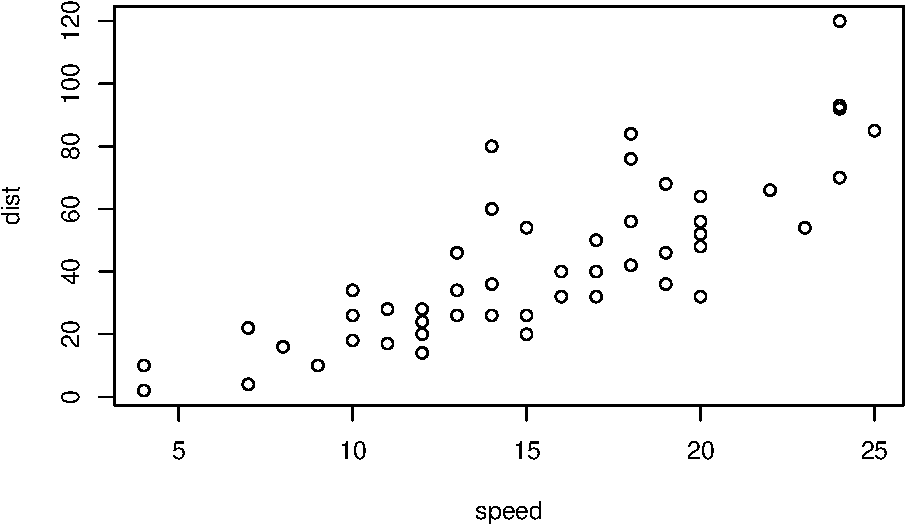
\includegraphics{skeleton_files/figure-latex/cars-1.pdf}
\caption{cars plot}
\end{figure}

\begin{Shaded}
\begin{Highlighting}[]
\FunctionTok{plot}\NormalTok{(mpg }\SpecialCharTok{\textasciitilde{}}\NormalTok{ hp, mtcars)}
\end{Highlighting}
\end{Shaded}

\begin{figure}
\centering
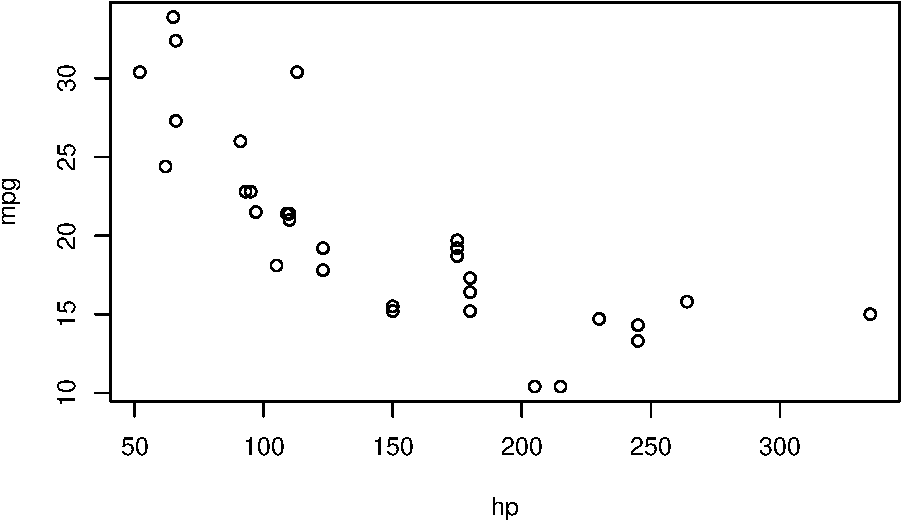
\includegraphics{skeleton_files/figure-latex/mtcars-1.pdf}
\caption{mtcars plot}
\end{figure}

\begin{longtable}[]{@{}lrr@{}}
\toprule
Species & Sepal\_Length\_Mean & Sepal\_Width\_Mean \\
\midrule
\endhead
setosa & 5.006 & 3.428 \\
versicolor & 5.936 & 2.770 \\
virginica & 6.588 & 2.974 \\
\bottomrule
\end{longtable}

\texttt{knitr::kable()} is now unusable (please check the issue:
https://github.com/rstudio/rticles/issues/93). I will modify the package
Tsukubamd BP asap.

\chapter*{General Discussion}
\addcontentsline{toc}{chapter}{General Discussion}\parindent=5.3mm

\chapter*{Acknowledgement}

The authors gratefully acknowledge \ldots{}

\chapter*{References}

\hypertarget{refs}{}
\begin{CSLReferences}{1}{0}
\leavevmode\vadjust pre{\hypertarget{ref-darwin2004origin}{}}%
Darwin, Charles. 2004. \emph{On the Origin of Species, 1859}. Routledge.

\leavevmode\vadjust pre{\hypertarget{ref-smith1993theory}{}}%
Smith, John Maynard, and Smith John Maynard. 1993. \emph{The Theory of
Evolution}. Cambridge University Press.

\leavevmode\vadjust pre{\hypertarget{ref-winfree1975unclocklike}{}}%
Winfree, Arthur T. 1975. {``Unclocklike Behaviour of Biological
Clocks.''} \emph{Nature} 253 (5490): 315--19.

\end{CSLReferences}

\bibliographystyle{agsm}
\bibliography{bibliography.bib}

\end{document}
